\documentclass[10pt]{exam}
\usepackage[phy]{template-for-exam}
\usepackage{multirow}
\usepackage{tikz}
\usetikzlibrary{shadings,decorations.pathmorphing,arrows.meta}
%\printanswers
\shadedsolutions
\renewcommand{\solutiontitle}{}

\title{Marble Lab -- Revisited \\ (KE and PE)}
\author{Rohrbach}
\date{\today}

\begin{document}
\maketitle

\newcommand{\ansbox}[1]{
  \begin{flushright}
    \begin{tabular}{|p{15em}|}
      \hline
      \\
      #1 \\
      \\
      \hline
    \end{tabular}
  \end{flushright}
}

\begin{solution}
  \begin{center}
      \Large \bf \color{red} 
      Makeup Version if absent.  Data is provided
  \end{center}
\end{solution}


\begin{center}
  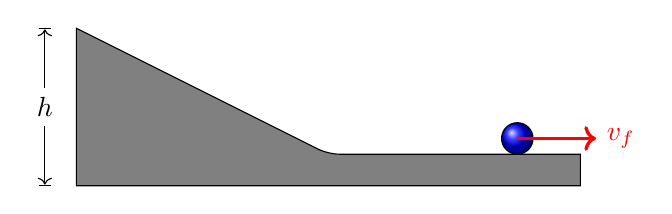
\begin{tikzpicture}[scale=4]
    \draw[fill=gray] (3,1.9)
      -- ++(0,-.1)
      -- ++(-1.6,0) 
      -- ++(0,0.5)
      to[rounded corners] ++(.8,-.4)
      -- cycle;
    \draw[shading=ball] (2.8,1.95) circle (0.05);
    \draw[->, very thick, red] (2.8,1.95) -- ++(.25,0) 
      node[anchor=west] {$v_f$};
    \draw[|<->|] (1.3,1.8) -- ++ (0,.5) 
      node[midway, fill=white] {$h$};
  
  \end{tikzpicture}
\end{center}

\begin{questions}
  
\question \label{height}
  Measure the height of the track ($h$): 
  \fillin[\color{red}20][7em] cm.  Convert it to meters.

  \ansbox{$h=$ \fillin[][7em] m}

\question \label{mass}
  Measure the mass of the marble ($m$): 
  \fillin[\color{red} 11][7em] g.  Convert it to kg.
  
  \ansbox{$m=$ \fillin[][7em] kg}

\question \label{prediction}
  Look at the four tracks on your ramp.  Assuming that there was no friction, which ramp do you think would cause the marble to go fastest?  Why?

  \begin{solution}[10em]
    {\color{red} \bf You can skip this question}
  \end{solution}

\question \label{expected-first}
  Calculate the speed of the marble at the bottom of the ramp.  Assume that there is no friction!
  \vs

  \ansbox{
    $v_f=$ \fillin[][7em] m/s \\ 
    \hfill \small (\emph{expected})
  }
  
\pagebreak

\question \label{data}
  Okay, let's measure it!  Put the photogate at the bottom of each track to measure the speed of the marble.

  \newcommand{\datatable}[2]{
    \renewcommand{\arraystretch}{1.5}
    \begin{tabular}{|c|p{5em}|}
      \hline
      \centering\arraybackslash Track & 
      \centering\arraybackslash Measured Velocity (m/s) \\
      \hline
      \ifprintanswers
        \multirow[c]{5}{*}{#1} & xxxx \\ \cline{2-2}
        & xxxx \\ \cline{2-2}
        & xxxx \\ \cline{2-2}
        & xxxx \\ \cline{2-2}
        & xxxx \\ \hline\hline
        Avg. & \bf\color{red}  #2 \\ \hline
      \else
        \multirow[c]{5}{*}{#1} & \\ \cline{2-2}
        &\\ \cline{2-2}
        &\\ \cline{2-2}
        &\\ \cline{2-2}
        &\\ \hline\hline
        Avg. &  \\ \hline
      \fi
    \end{tabular}
    \renewcommand{\arraystretch}{1}
  }

  \datatable{Red}{1.53} 
  \datatable{Blue}{1.43}
  \datatable{Yellow}{1.45}
  \datatable{Green}{1.51}

\question
  Look at the prediction you made in questions \#\ref{prediction}. Was it correct? 

  \begin{solution}[\stretch{1}]
    {\color{red} \bf You can skip this question}
  \end{solution}
 
\question \label{measured}
  The final velocity should have been pretty consistent down each track.  Calculate the average final velocity across all the tracks.

  \ansbox{
    $v_f=$ \fillin[][7em] m/s \\ 
    \hfill \small (\emph{measured})
  }

\question
  Calculate the percent error of your measured average velocity (see \#\ref{measured}) compared to the expected velocity (see \#\ref{expected-first}).
  %
  \begin{align*}
    \text{\% error} &=  
    \frac{
      \left|\text{measured}-\text{expected}\right|
      }{
        \text{expected}
      } 
    \times 100
  \end{align*}
  %
  \vs 

\question
  Comment on this percentage.  Does it seem like your results are accurate?
  \vs 

\question \label{rolling-work}
  You should notice that percent error is pretty large.  It turns out that it takes quite a large amount of work to make the marble start rolling.  As a matter of fact, the work is 40\% of the starting initial potential energy.  It is also negative because it is taking energy out of the system.  Go ahead and calculate the work needed to make the marble roll:
  %
  \begin{align*}
    W &= -0.40 \times mgh_i
  \end{align*}
  %
  \vs  

\pagebreak


\question \label{expected-second}
  Now, let's try our calculation again.  Using the work you found in problem \#\ref{rolling-work}, and the initial height you found way back in \#\ref{height}, calculate the final velocity of the marble.
  \vs[2] 

  \ansbox{
    $v_f=$ \fillin[][7em] m/s \\ 
    \hfill \small (\emph{expected})
  }

\question 
  Calculate the percent error of your measured average velocity (see \#\ref{measured}) compared to the expected velocity (see \#\ref{expected-second}).
  %
  \begin{align*}
    \text{\% error} &=  
    \frac{
      \left|\text{measured}-\text{expected}\right|
      }{
        \text{expected}
      } 
    \times 100
  \end{align*}
  %
  \vs 

\question
  Comment on this percentage.  Now, does it seem like your results are accurate?
  \vs 

\question
  {\bf Conclusion:} Explain in detail what happened to the energy of the marble as it went down the ramp and how the lab showed the concept of energy conservation.
  \vs


\end{questions}

\end{document}